%DIF 1-2d1
%DIF LATEXDIFF DIFFERENCE FILE
%DIF DEL ../rom_sciAdvances.tex    Sun Nov 18 07:30:14 2018
%DIF ADD rom_sciAdvances_rev.tex   Thu Dec 20 11:40:11 2018
%DIF < % Use only LaTeX2e, calling the article.cls class and 12-point type.
%DIF < 
%DIF -------
\documentclass[12pt]{article}

%DIF 5-10d3
%DIF < % Users of the {thebibliography} environment or BibTeX should use the
%DIF < % scicite.sty package, downloadable from *Science* at
%DIF < % http://www.sciencemag.org/authors/preparing-manuscripts-using-latex 
%DIF < % This package should properly format in-text
%DIF < % reference calls and reference-list numbers.
%DIF < 
%DIF -------
\usepackage{scicite}
\let\citep=\cite

% \usepackage{times}

%DIF 16-20d8
%DIF < % The preamble here sets up a lot of new/revised commands and
%DIF < % environments.  It's annoying, but please do *not* try to strip these
%DIF < % out into a separate .sty file (which could lead to the loss of some
%DIF < % information when we convert the file to other formats).  Instead, keep
%DIF < % them in the preamble of your main LaTeX source file.
%DIF -------

\usepackage{graphicx}
\usepackage{authblk}
\usepackage{lineno}
\usepackage{paralist}
\usepackage{amsmath}

%DIF 28-33d15
%DIF < %% for citing stuff in the supp
%DIF < % \usepackage{xr}
%DIF < % \externaldocument{rom_sciAdvances_supp}
%DIF < 
%DIF < % The following parameters seem to provide a reasonable page setup.
%DIF < 
%DIF -------
\topmargin 0.0cm
\oddsidemargin 0.2cm
\textwidth 16cm 
\textheight 21cm
\footskip 1.0cm


%DIF 41-42c22
%DIF < %The next command sets up an environment for the abstract to your paper.
%DIF < 
%DIF -------
% environment for the abstract %DIF > 
%DIF -------
\newenvironment{sciabstract} 
{\bfseries}
{}

% to include rmd output
\usepackage[final]{pdfpages}



%DIF 48a28-33
\title{Non-equilibrium evolution of volatility in origination and %DIF > 
  extinction explains fat-tailed fluctuations in Phanerozoic %DIF > 
  biodiversity \\ %DIF > 
  \vspace{1em} \large {\it One sentence summary:} Phanerozoic marine %DIF > 
  invertebrate richness fluctuates in a non-equilibrium process due to %DIF > 
  pulsed adaptive evolution.} %DIF > 
%DIF -------

%DIF 49-53d35
%DIF < % Include your paper's title here
%DIF < 
%DIF < \title{Non-equilibrium rate heterogeneity explains fat-tailed
%DIF <   fluctuations in Phanerozoic biodiversity}
%DIF < 
%DIF -------
\author[1, {*}]{Andrew J. Rominger}
\author[1, 2, 3]{Miguel A. Fuentes}
\author[1, 4, 5, 6, 7]{Pablo A. Marquet}

\affil[1]{\normalsize{Santa Fe Institute, 1399 Hyde Park Road, Santa Fe, New
Mexico 87501, US}}
%
\affil[2]{\normalsize{Instituto de Investigaciones Filos\'oficas, SADAF, CONICET,
Bulnes 642, 1428 Buenos Aires, Argentin}}
%
\affil[3]{\normalsize{Facultad de Ingenier\'ia y Tecnolog\'ia, Universidad San
Sebasti\'an, Lota 2465, Santiago 7510157, Chile}}
%
\affil[4]{\normalsize{Departamento de Ecolog\'ia, Facultad de Ciencias
Biol\'ogicas, Pontificia Universidad de Chile, Alameda 340, Santiago,
Chile}}
%
%DIF 71-72c52-53
%DIF < \affil[5]{\normalsize{Instituto de Ecolog\'ia y Biodiversidad, Casilla 653,
%DIF < Santiago, Chile}}
%DIF -------
\affil[5]{\normalsize{Instituto de Ecolog\'ia y Biodiversidad (IEB), %DIF > 
    Casilla 653, Santiago, Chile}} %DIF > 
%DIF -------
%
%DIF 74-76c55-57
%DIF < \affil[6]{\normalsize{Laboratorio Internacional de Cambio Global (LINCGlobal),
%DIF < Pontificia Universidad Católica de Chile, Alameda 340, Santiago,
%DIF < Chile}}
%DIF -------
\affil[6]{\normalsize{Laboratorio Internacional de Cambio Global %DIF > 
    (LINCGlobal), and Centro de Cambio Global UC, Pontificia %DIF > 
    Universidad Catolica de Chile, Santiago, Chile.}} %DIF > 
%DIF -------
%
%DIF 78-79c59-60
%DIF < \affil[7]{\normalsize{Centro Cambio Global UC, Av.~Vicu\~na Mackenna 4860, Campus
%DIF < San Vicu\~na, Santiago, Chile}}
%DIF -------
\affil[7]{\normalsize{Centro Cambio Global UC, Av.~Vicu\~na Mackenna %DIF > 
    4860, Campus San Vicu\~na, Santiago, Chile}} %DIF > 
%DIF -------
%
%DIF 81c62-66
%DIF < \affil[{*}]{\normalsize{To whom correspondence should be addressed; E-mail: rominger@santafe.edu}}
%DIF -------
\affil[8]{\normalsize{Centro de Ciencias de la Complejidad (C3), %DIF > 
    Universidad Nacional Aut\'onoma de M\'exico.}} %DIF > 
% %DIF > 
\affil[{*}]{\normalsize{To whom correspondence should be addressed, %DIF > 
    e-mail: rominger@santafe.edu}} %DIF > 
%DIF -------

\date{}



%DIF < %%%%%%%%%%%%%%%%% END OF PREAMBLE %%%%%%%%%%%%%%%%
%DIF -------
%%%% END OF PREAMBLE %%%% %DIF > 
%DIF PREAMBLE EXTENSION ADDED BY LATEXDIFF
%DIF UNDERLINE PREAMBLE %DIF PREAMBLE
\RequirePackage[normalem]{ulem} %DIF PREAMBLE
\RequirePackage{color}\definecolor{RED}{rgb}{1,0,0}\definecolor{BLUE}{rgb}{0,0,1} %DIF PREAMBLE
\providecommand{\DIFadd}[1]{{\color{blue}{#1}}} %DIF PREAMBLE
\providecommand{\DIFdel}[1]{{\protect\color{red}\sout{}}}                      %DIF PREAMBLE
%DIF SAFE PREAMBLE %DIF PREAMBLE
\providecommand{\DIFaddbegin}{} %DIF PREAMBLE
\providecommand{\DIFaddend}{} %DIF PREAMBLE
\providecommand{\DIFdelbegin}{} %DIF PREAMBLE
\providecommand{\DIFdelend}{} %DIF PREAMBLE
%DIF FLOATSAFE PREAMBLE %DIF PREAMBLE
\providecommand{\DIFaddFL}[1]{\DIFadd{#1}} %DIF PREAMBLE
\providecommand{\DIFdelFL}[1]{\DIFdel{#1}} %DIF PREAMBLE
\providecommand{\DIFaddbeginFL}{} %DIF PREAMBLE
\providecommand{\DIFaddendFL}{} %DIF PREAMBLE
\providecommand{\DIFdelbeginFL}{} %DIF PREAMBLE
\providecommand{\DIFdelendFL}{} %DIF PREAMBLE
\newcommand{\DIFscaledelfig}{0.5}
%DIF HIGHLIGHTGRAPHICS PREAMBLE %DIF PREAMBLE
\RequirePackage{settobox} %DIF PREAMBLE
\RequirePackage{letltxmacro} %DIF PREAMBLE
\newsavebox{\DIFdelgraphicsbox} %DIF PREAMBLE
\newlength{\DIFdelgraphicswidth} %DIF PREAMBLE
\newlength{\DIFdelgraphicsheight} %DIF PREAMBLE
% store original definition of \includegraphics %DIF PREAMBLE
\LetLtxMacro{\DIFOincludegraphics}{\includegraphics} %DIF PREAMBLE
\newcommand{\DIFaddincludegraphics}[2][]{{\color{blue}\fbox{\DIFOincludegraphics[#1]{#2}}}} %DIF PREAMBLE
\newcommand{\DIFdelincludegraphics}[2][]{% %DIF PREAMBLE
\sbox{\DIFdelgraphicsbox}{\DIFOincludegraphics[#1]{#2}}% %DIF PREAMBLE
\settoboxwidth{\DIFdelgraphicswidth}{\DIFdelgraphicsbox} %DIF PREAMBLE
\settoboxtotalheight{\DIFdelgraphicsheight}{\DIFdelgraphicsbox} %DIF PREAMBLE
\scalebox{\DIFscaledelfig}{% %DIF PREAMBLE
\parbox[b]{\DIFdelgraphicswidth}{\usebox{\DIFdelgraphicsbox}\\[-\baselineskip] \rule{\DIFdelgraphicswidth}{0em}}\llap{\resizebox{\DIFdelgraphicswidth}{\DIFdelgraphicsheight}{% %DIF PREAMBLE
\setlength{\unitlength}{\DIFdelgraphicswidth}% %DIF PREAMBLE
\begin{picture}(1,1)% %DIF PREAMBLE
\thicklines\linethickness{2pt} %DIF PREAMBLE
{\color[rgb]{1,0,0}\put(0,0){\framebox(1,1){}}}% %DIF PREAMBLE
{\color[rgb]{1,0,0}\put(0,0){\line( 1,1){1}}}% %DIF PREAMBLE
{\color[rgb]{1,0,0}\put(0,1){\line(1,-1){1}}}% %DIF PREAMBLE
\end{picture}% %DIF PREAMBLE
}\hspace*{3pt}}} %DIF PREAMBLE
} %DIF PREAMBLE
\LetLtxMacro{\DIFOaddbegin}{\DIFaddbegin} %DIF PREAMBLE
\LetLtxMacro{\DIFOaddend}{\DIFaddend} %DIF PREAMBLE
\LetLtxMacro{\DIFOdelbegin}{\DIFdelbegin} %DIF PREAMBLE
\LetLtxMacro{\DIFOdelend}{\DIFdelend} %DIF PREAMBLE
\DeclareRobustCommand{\DIFaddbegin}{\DIFOaddbegin \let\includegraphics\DIFaddincludegraphics} %DIF PREAMBLE
\DeclareRobustCommand{\DIFaddend}{\DIFOaddend \let\includegraphics\DIFOincludegraphics} %DIF PREAMBLE
\DeclareRobustCommand{\DIFdelbegin}{\DIFOdelbegin \let\includegraphics\DIFdelincludegraphics} %DIF PREAMBLE
\DeclareRobustCommand{\DIFdelend}{\DIFOaddend \let\includegraphics\DIFOincludegraphics} %DIF PREAMBLE
\LetLtxMacro{\DIFOaddbeginFL}{\DIFaddbeginFL} %DIF PREAMBLE
\LetLtxMacro{\DIFOaddendFL}{\DIFaddendFL} %DIF PREAMBLE
\LetLtxMacro{\DIFOdelbeginFL}{\DIFdelbeginFL} %DIF PREAMBLE
\LetLtxMacro{\DIFOdelendFL}{\DIFdelendFL} %DIF PREAMBLE
\DeclareRobustCommand{\DIFaddbeginFL}{\DIFOaddbeginFL \let\includegraphics\DIFaddincludegraphics} %DIF PREAMBLE
\DeclareRobustCommand{\DIFaddendFL}{\DIFOaddendFL \let\includegraphics\DIFOincludegraphics} %DIF PREAMBLE
\DeclareRobustCommand{\DIFdelbeginFL}{\DIFOdelbeginFL \let\includegraphics\DIFdelincludegraphics} %DIF PREAMBLE
\DeclareRobustCommand{\DIFdelendFL}{\DIFOaddendFL \let\includegraphics\DIFOincludegraphics} %DIF PREAMBLE
%DIF END PREAMBLE EXTENSION ADDED BY LATEXDIFF

\begin{document} 

\setcounter{page}{1}
\nolinenumbers

\newcommand{\beginsupplement}{%
  \setcounter{table}{0}
  \renewcommand{\thetable}{S\arabic{table}}%
  \setcounter{figure}{0}
  \renewcommand{\thefigure}{S\arabic{figure}}%
  \setcounter{section}{0}
  \renewcommand{\thesection}{S\arabic{section}}%
}

\beginsupplement

\begin{center}
{\LARGE \bf Supplementary materials}
\end{center}
\vspace{2em}

\section{Limit distribution of a time-averaged homogeneous
  origination-extinction process}
\label{sec:suppLimitDist}
\DIFaddbegin 

\DIFaddend Fossil taxa gain and lose \DIFdelbegin \DIFdel{taxa }\DIFdelend \DIFaddbegin \DIFadd{genera }\DIFaddend according to an
origination-extinction process. We assume that most fossil occurrences
of a taxon come from the period of its history when it is dominant and
in steady state. In a time slice of duration $\tau$ during such a
period of steady state the latent per capita rates of origination and
extinction would be equal (i.e. $\lambda = \mu \equiv \rho$) and the
number of origination or extinctions events (call such events $Y$)
each follow an inhomogeneous Poisson process with rate $\rho N_t$
where $N_t$ is the number of \DIFdelbegin \DIFdel{species or }\DIFdelend genera in the taxon of interest at time
$t$. Allowing $N_t$ to vary smoothly with time, and \DIFdelbegin \DIFdel{invoking the communicative property of the Poisson distribution}\DIFdelend \DIFaddbegin \DIFadd{recognizing that
the sum of Poisson random variables remains Poisson}\DIFaddend , we arrive at the
number $Y$ of extinction \emph{or} origination events in $\tau$ being
distributed
\begin{equation}
  \label{eq:eventPois1}
  Y \sim \text{Pois}\left(\rho \int_{t=0}^\tau N(t) dt\right).
\end{equation}
Under the steady state assumption we can approximate $N(t)$ by
$\bar{N}$, the steady state \DIFdelbegin \DIFdel{diversity}\DIFdelend \DIFaddbegin \DIFadd{richness}\DIFaddend , leading to
\begin{equation}
  \label{eq:eventPois2}
  Y \sim \text{Pois}(\rho \bar{N} \tau).
\end{equation}

\DIFdelbegin \DIFdel{Assuming the $\tau$ of each time period in the Paleobiology Database
or Sepkoski's compendium to be approximately equal (i. e. equal
durations of major asymptotic units) then the }\DIFdelend \DIFaddbegin \DIFadd{This Poisson distribution is asymptotically Gaussian, which is a more
appropriate distribution for our sampling and bias-corrected richness
estimates because these estimates are not integer-valued but rather
continuous random variables. Furthermore, because we use standard time
periods of average duration $\tau = 11\text{MY}$ the the }\DIFaddend distribution
of fluctuations within taxa will be \DIFaddbegin \DIFadd{independent of the specific time
periods considered. }\DIFaddend The Gaussian asymptotics of time-averaged
birth-death processes have been proven and explored elsewhere as well
\DIFdelbegin \DIFdel{\mbox{%DIFAUXCMD
\citep{keilson1970,
  grassmann1987}}%DIFAUXCMD
}\DIFdelend \DIFaddbegin \DIFadd{\mbox{%DIFAUXCMD
\citep{grassmann1987}}%DIFAUXCMD
}\DIFaddend .


\section{\DIFadd{Evaluation of sampling bias correction methods}}
\label{sec:suppBiasEval}

\DIFaddbegin \DIFadd{Our sampling and bias-correction method first accounts for imperfect
detection within a binomial sampling framework as described in the
main text, and then further corrects for potential publication bias
using simple log-log regression.  We reproduce that regression of
log-richness versus log-number of publications here
(Fig. \ref{figSupp:divByPub}). }\DIFaddend 

\DIFaddbegin \begin{figure}[!hp]
  \centering
  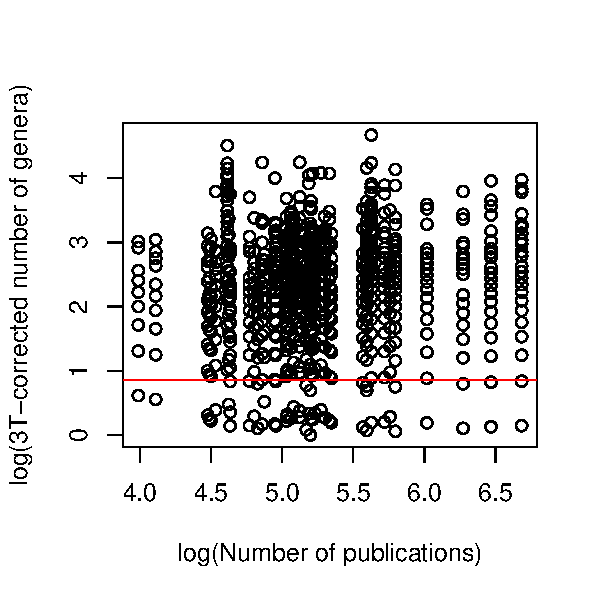
\includegraphics[width=0.4\textwidth]{../../figSupp_divByPub.pdf}
  \caption{\DIFaddFL{Relationship between number of publications and genus
    richness at the family level as recorded by the PBDB.}}
  \label{figSupp:divByPub}
\end{figure}


\DIFadd{We compare our sampling and bias-correction method to other more
established approaches. Specifically we use the newly available R
package }{\it \DIFadd{divDyn}} \DIFadd{\mbox{%DIFAUXCMD
\citep{kocsis2018} }%DIFAUXCMD
to produce subsampling-based
richness estimates for the Phanerozoic timeseries of marine
invertebrates. In Figure \ref{figSupp:3TPub} we compare classical
rarefaction and shareholder quorum subsampling (SQS) with our
method. All samples were rarified to 120 occurrences, which is
approximately the maximum possible rarefied sample size across all
time bins, and the SQS quorum was set to 0.75 to similarly approximate
this common sampling denominator across time bins. For both
rarefaction and SQS we averaged 50 subsampled replicates.}\DIFaddend 


\DIFaddbegin \begin{figure}[!hp]
  \centering
  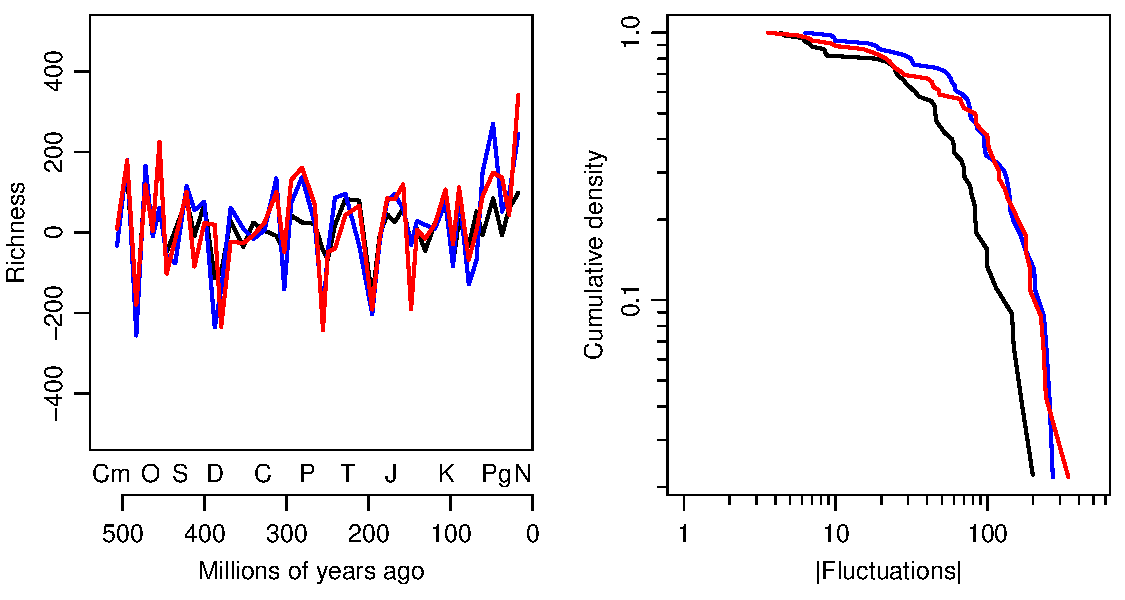
\includegraphics[width=0.7\textwidth]{../../figSupp_divEstComp.pdf}
  \caption{\DIFaddFL{Comparison of rarefaction (black line) and SQS (blue)
    with our three-timer and publication bias correction method
    (red). The time-series of all marine invertebrate genera shows
    general agreement with the only major deviations toward the modern
    (A). Despite these differences the distribution of fluctuations in
    genus richness across all marine invertebrates show good agreement
    (B).}}
  \label{figSupp:3TPub}
\end{figure}


\section{\DIFadd{Understanding deviations from superstatistics at higher
  taxonomic levels}}
\label{sec:suppSstatTaxLevels}

\DIFadd{To explore why deviations from super statistics increase with
increasing taxonomic level we explore how the distributions of
richness fluctuations $p_k(x | \beta_k)$ and fluctuation volatilities
$f(\beta_k)$ change with changing taxonomic level. We find that
richness fluctuation distributions experience increasing frequencies
of outliers (increasing kurtosis) with higher taxonomic level
(Fig. \ref{figSupp:pkx_allTaxa}). We also find that observed
fluctuation volatility distributions increasingly depart from a Gamma
distribution at the levels of classes and phyla
(Fig. \ref{figSupp:fbeta_allTaxa}).}\DIFaddend 


\DIFaddbegin \begin{figure}[!hp]
  \centering
  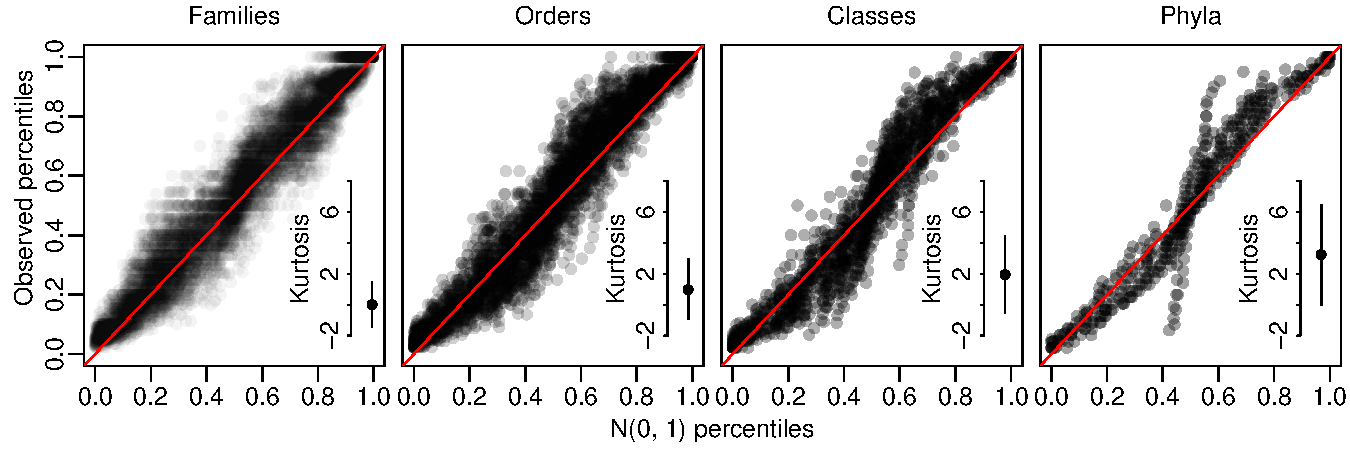
\includegraphics[width=0.8\textwidth]{../../figSupp_pkx_allTaxa.pdf}
  \caption{\DIFaddFL{Change in within clade richness fluctuation distributions
    with increasing taxonomic level. The percentile-percentile plots
    show how the percentiles of observed re-scaled fluctuation
    distributions compare to expected percentiles from a Gaussian
    distribution with mean 0 and variance 1. We can see that families
    conform to a linear relationship while higher taxa, even at the
    order level, begin to show s-shaped relationships. Inset plots
    show how kurtosis increases from 0 (the value for a Gaussian
    distribution) at the family level to increasingly larger values
    at higher taxonomic levels.}}
  \label{figSupp:pkx_allTaxa}
\end{figure}

\DIFaddbegin \begin{figure}[!hp]
  \centering
  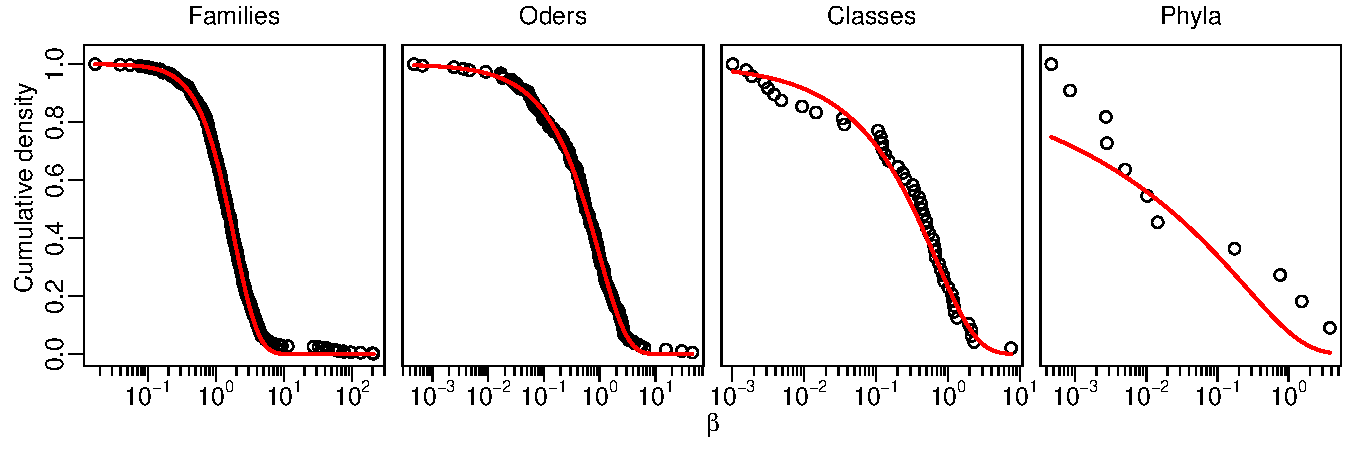
\includegraphics[width=0.8\textwidth]{../../figSupp_fbeta_allTaxa.pdf}
  \caption{\DIFaddFL{Change in the distributions of $\beta_k$ across clades of
    increasing taxonomic level. Points are observed $\beta_k$ values
    and red lines are the best-fit Gamma distributions. Deviations
    increase particularly at the class and phylum levels.}}
  \label{figSupp:fbeta_allTaxa}
\end{figure}




\DIFaddbegin \section{\DIFadd{Ecospace occupation of higher taxa}}
\label{sec:suppGuilds} 

\DIFadd{We posit that part of the increasing divergence between
superstatistics and observed fluctuations and the increase in
fluctuation outliers at higher taxonomic levels is that these higher
taxa increasingly aggregate disparate types of organisms. One way to
evaluate this idea is to count the ecospace hypercubes
\mbox{%DIFAUXCMD
\citep{bambach1983, bambach2007, bush2007} }%DIFAUXCMD
occupied by taxa at
different levels. We use the ecological characteristics reported by
the PBDB: taxon environment, motility, life habit, vision, diet,
reproduction, and ontogeny. In Figure \ref{figSupp:eeSpaceOcc} we find
that families comprise, on average, 1 hypercube, families comprise 2
hypercubes on average, and classes and phyla comprise many more.}


\DIFaddbegin \begin{figure}[!hp]
  \centering
  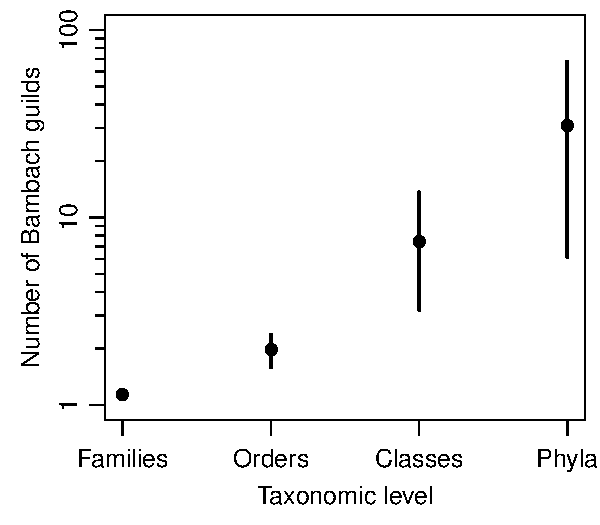
\includegraphics[width=0.4\textwidth]{../../figSupp_eeSpaceOcc.pdf} 
  \caption{\DIFaddFL{Relationship between number of ecospace hypercubes occupied
    and taxonomic level.}}
  \label{figSupp:eeSpaceOcc}
\end{figure}


\section{\DIFadd{Relationship between $\beta_k$ and clade richness}}
\label{sec:suppBetaRichness} 

\DIFadd{There is likely to be a relationship between richness of clade $k$ and
its fluctuation volatility $\beta_k$ because both extinction and
origination (i.e. the formation of new genera) contribute to
volatility. Thus we expect that higher variance in richness
fluctuations (i.e. smaller $\beta_k = 1/\text{variance}$) will be
correlated with higher richness.  Indeed, Figure
\ref{figSupp:betaByRich} shows this to be true. In the main text we
use permutation to evaluate whether this correlation is responsible
for the observed good fit of superstatistics, and find that this
correlation alone is not sufficient.
}

\DIFaddbegin \begin{figure}[!hp]
  \centering
  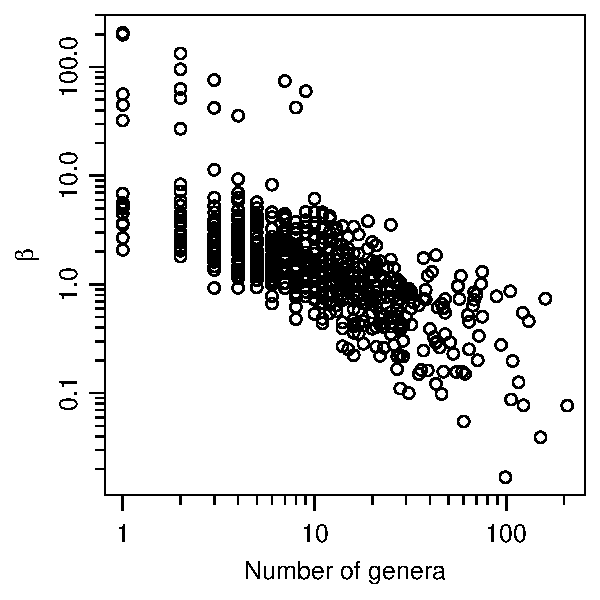
\includegraphics[width=0.4\textwidth]{../../figSupp_betaByRich.pdf} 
  \caption{\DIFaddFL{Relationship between fluctuation volatility $\beta_k$ and
    genus richness at the family level.}}
  \label{figSupp:betaByRich}
\end{figure}


\clearpage 

\setlength{\voffset}{0cm}
\setlength{\hoffset}{0cm}
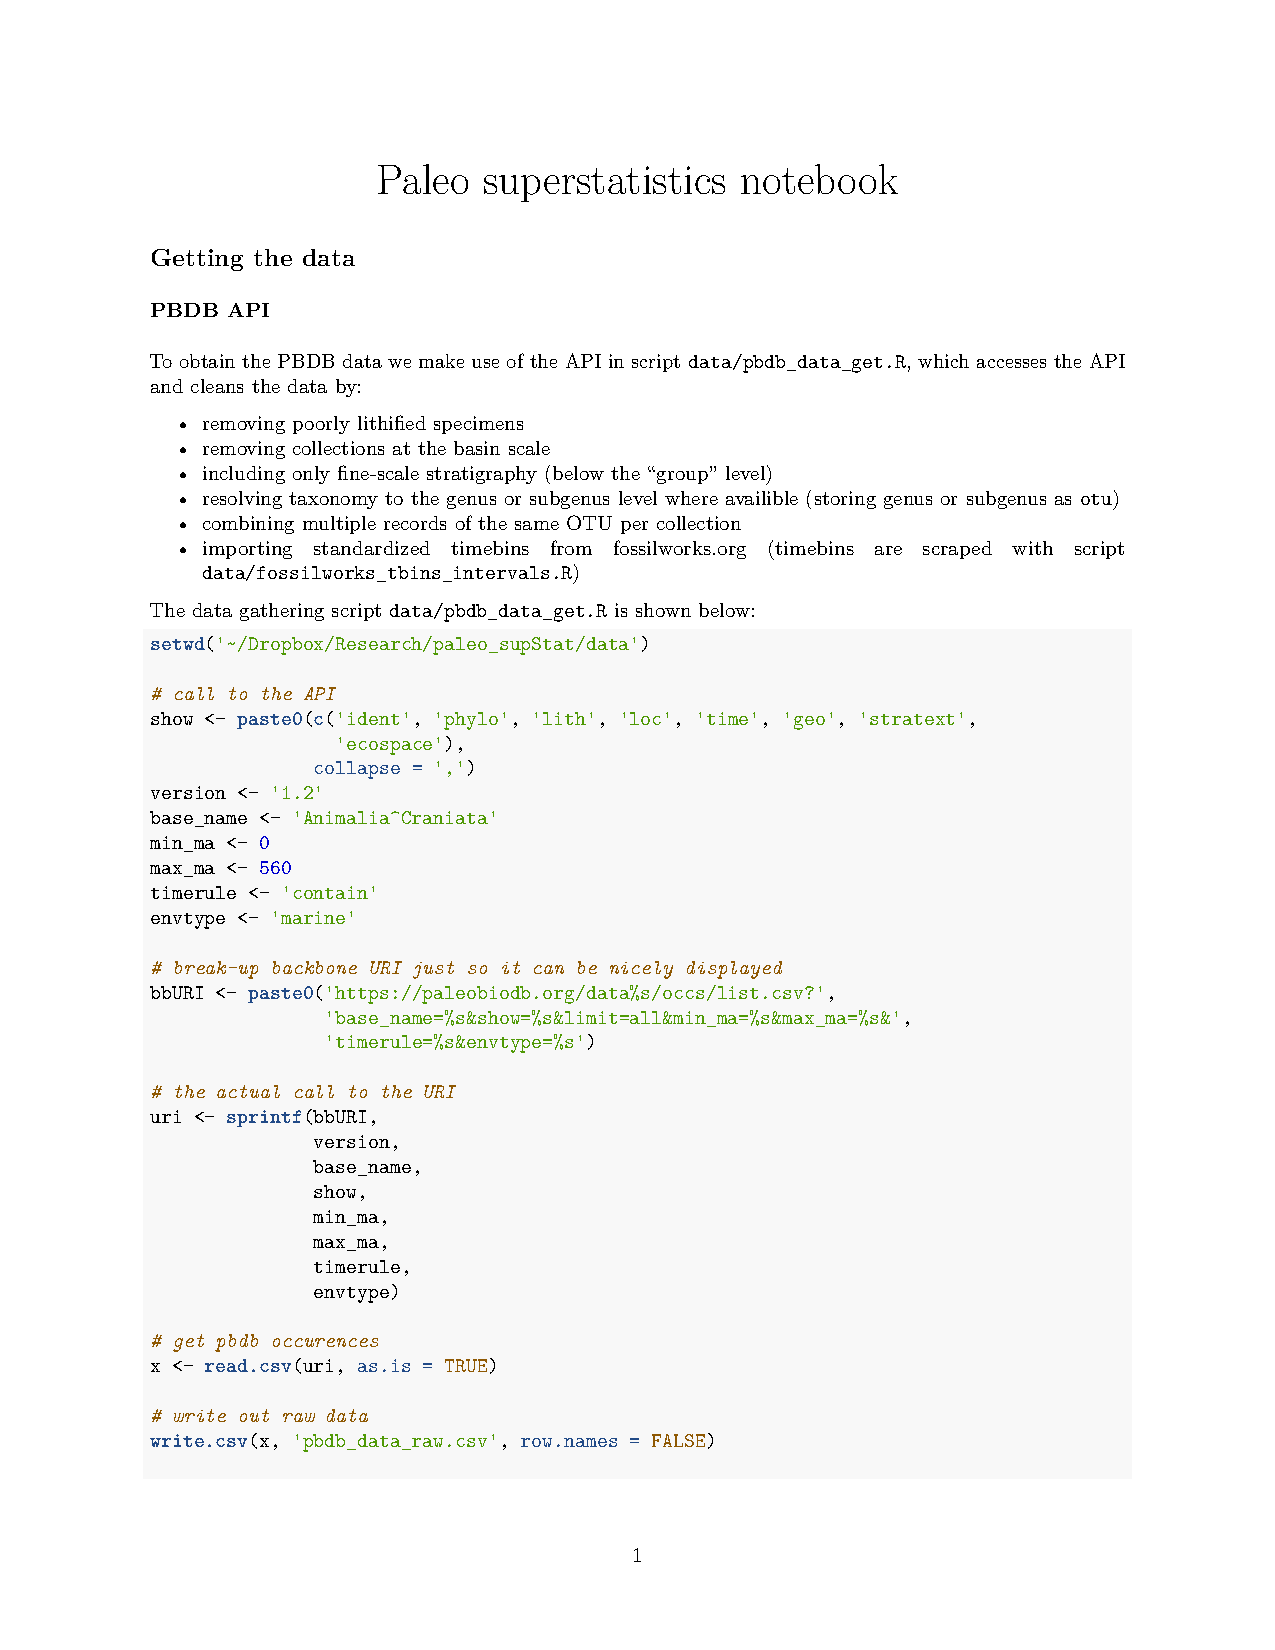
\includepdf[pages=-]{../../../sstat_notebook.pdf}

% \input{../../../sstat_notebook_include.tex}
\end{document}

